
%%%%%%%%%%%%%%%%%%%%%%%%%%%%%%%%%%%%%%%%%
% Beamer Presentation
% LaTeX Template
% Version 1.0 (10/11/12)
%
% This template has been downloaded from:
% http://www.LaTeXTemplates.com
%
% License:
% CC BY-NC-SA 3.0 (http://creativecommons.org/licenses/by-nc-sa/3.0/)
%
%%%%%%%%%%%%%%%%%%%%%%%%%%%%%%%%%%%%%%%%%

%----------------------------------------------------------------------------------------
%	PACKAGES AND THEMES
%----------------------------------------------------------------------------------------

\documentclass[12pt,usenames,dvipsnames]{beamer}

\mode<presentation> {

% The Beamer class comes with a number of default slide themes
% which change the colors and layouts of slides. Below this is a list
% of all the themes, uncomment each in turn to see what they look like.

%\usetheme{default}
%\usetheme{AnnArbor}
%\usetheme{Antibes}
%\usetheme{Bergen}
%\usetheme{Berkeley}
%\usetheme{Berlin}
%\usetheme{Boadilla}
%\usetheme{CambridgeUS}
%\usetheme{Copenhagen}
%\usetheme{Darmstadt}
%\usetheme{Dresden}
%\usetheme{Frankfurt}
%\usetheme{Goettingen}
%\usetheme{Hannover}
%\usetheme{Ilmenau}
%\usetheme{JuanLesPins}
%\usetheme{Luebeck}
%\usetheme{Madrid}
%\usetheme{Malmoe}
%\usetheme{Marburg}
%\usetheme{Montpellier}
%\usetheme{PaloAlto}
%\usetheme{Pittsburgh}
%\usetheme{Rochester}
%\usetheme{Singapore}
%\usetheme{Szeged}
%\usetheme{Warsaw}
\usetheme[secheader]{Boadilla}

% As well as themes, the Beamer class has a number of color themes
% for any slide theme. Uncomment each of these in turn to see how it
% changes the colors of your current slide theme.

%\usecolortheme{albatross}
%\usecolortheme{beaver}
%\usecolortheme{beetle}
%\usecolortheme{crane}
%\usecolortheme{dolphin}
%\usecolortheme{dove}
%\usecolortheme{fly}
%\usecolortheme{lily}
%\usecolortheme{orchid}
%\usecolortheme{rose}
%\usecolortheme{seagull}
%\usecolortheme{seahorse}
%\usecolortheme{whale}
%\usecolortheme{wolverine}

%\setbeamertemplate{footline} % To remove the footer line in all slides uncomment this line
%\setbeamertemplate{footline}[page number] % To replace the footer line in all slides with a simple slide count uncomment this line

\setbeamertemplate{navigation symbols}{} % To remove the navigation symbols from the bottom of all slides uncomment this line
}

\usepackage{graphicx} % Allows including images
\usepackage{tikz}
\usepackage{booktabs} % Allows the use of \toprule, \midrule and \bottomrule in tables
%\usepackage[font=small,skip=0pt]{caption}
\usepackage{cancel}
\usepackage{xcolor}

\newcommand\Ccancel[2][black]{\renewcommand\CancelColor{\color{#1}}\cancel{#2}}

\usepackage[config, labelfont={bf}]{caption,subfig} % nice sub figures
%\usepackage{enumitem}

\newcommand\parallelcontent[2]{
	\begin{columns}[t]
		\column{0.65\textwidth} #1
		\column{0.35\textwidth} #2
	\end{columns}
}
\newcommand\parallelitem[2]{
	\parallelcontent
	{\begin{itemize} \item #1 \end{itemize}}
	{\begin{itemize} \item #2 \end{itemize}}
}

\newcommand{\backupbegin}{
	\newcounter{finalframe}
	\setcounter{finalframe}{\value{framenumber}}
}
\newcommand{\backupend}{
	\setcounter{framenumber}{\value{finalframe}}
}

\newlength{\blockheight}
\setlength{\blockheight}{.95\textheight}
\newlength{\blockwidth}
\setlength{\blockwidth}{.95\textwidth}

\newenvironment{MRuleBlock}[3]{%
	\begin{minipage}[t][#2][t]{#3}%
		\begin{block}{#1}%
		}{%
		\end{block}%
	\end{minipage}%
}
%----------------------------------------------------------------------------------------
%	TITLE PAGE
%----------------------------------------------------------------------------------------
%\logo{
\includegraphics[width=0.05\textwidth]{../images/utlogo}}
\title[]{Cross Sections and EMC effect.} % The short title appears at the bottom of every slide, the full title is only on the title page

\author{Jason Bane} % Your name
\institute[UTK] % Your institution as it will appear on the bottom of every slide, may be shorthand to save space
{
University of Tennessee \\ % Your institution for the title page
\medskip
\textit{jbane1@vols.utk.edu} % Your email address
}
\date{} % Date, can be changed to a custom date
\captionsetup{font=small,skip=0pt}
\begin{document}


\begin{frame}
\titlepage % Print the title page as the first slide
\end{frame}

%------------------------------------------------------------------
\begin{frame}{}
	\begin{columns}
	\column{0.5\textwidth}
		\begin{block}{Monte Carlo}
			\begin{itemize}
				\item Generate events $\rightarrow$ Pass through magnetic apertures
				\item Tune Simulation offsets to match detector response
				\item Use model to weight events
				\begin{itemize}
					\item Deep Inelastic and resonance region from Ari Bodek Fit from E139 
					\item Full Mo and Tsai radiative correction
				\end{itemize}
			\end{itemize}
			\cite{bodek}  
			[L.W. Mo and Y.S. Tsai, 1969] 
		\end{block}
	\column{0.45\textwidth}
		\vspace{-20pt}
		\begin{figure}
			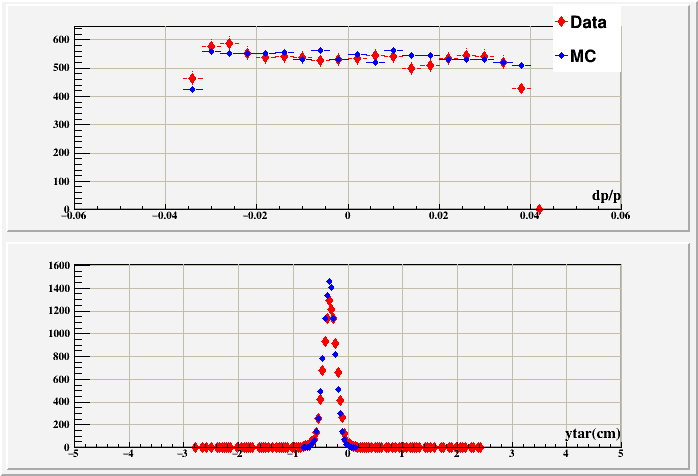
\includegraphics[width=6cm]{../images/dp_ytar_1207.png}
		\end{figure}
		\vspace{-30pt}
		\begin{figure}
			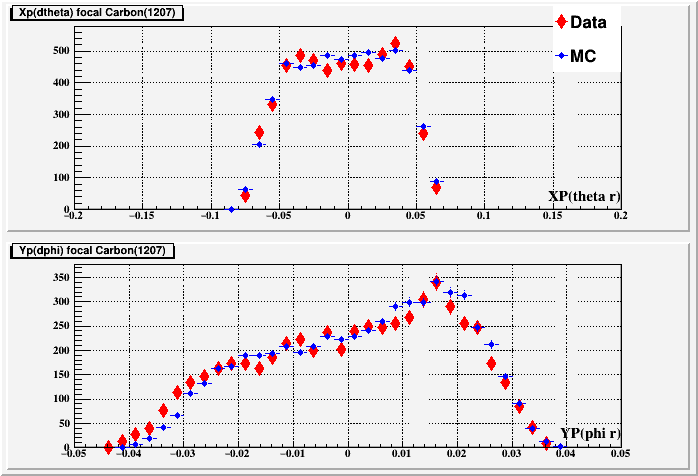
\includegraphics[width=6cm]{../images/xp_yp_foc_1207.png}
		\end{figure}
	\end{columns}
\end{frame}





\begin{frame}{Yield \& MC ratio D }
\vspace{-0.75cm}
\begin{figure}
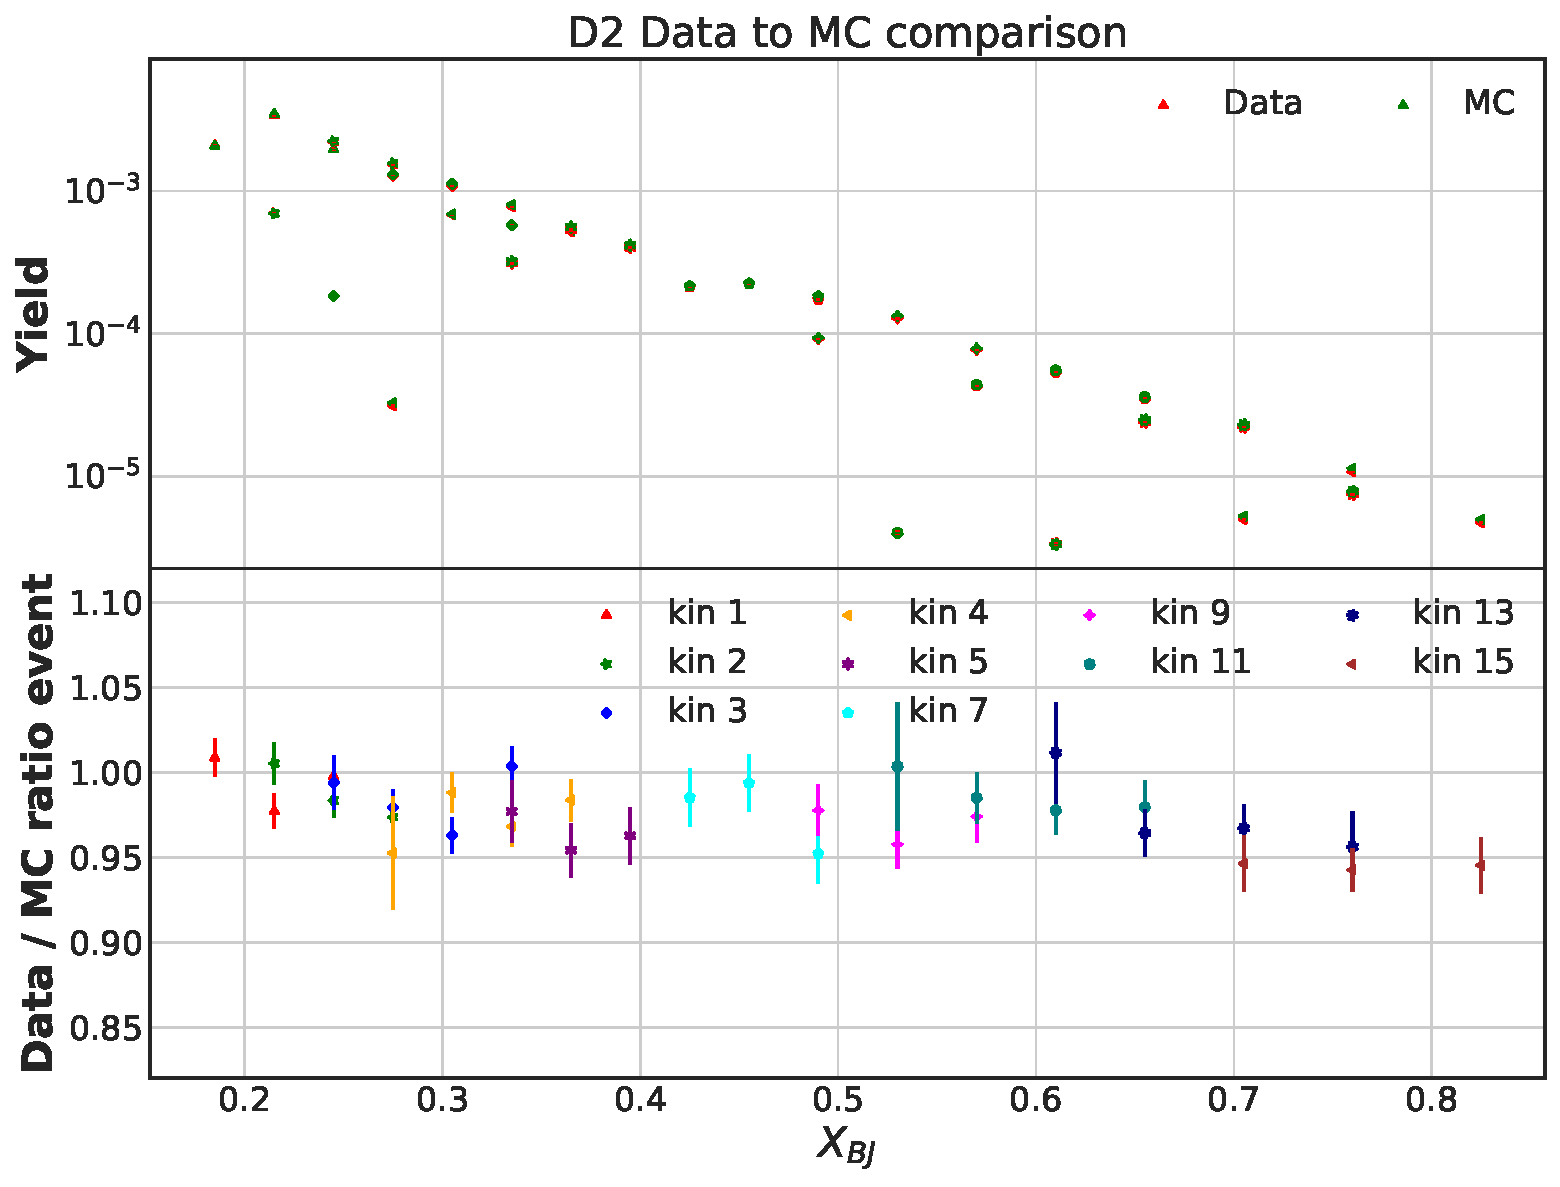
\includegraphics[width=12cm,height=8cm]{../images/D2yields.pdf}
\end{figure}
\end{frame}



\begin{frame}{}
\frametitle{DIS Cross Section}
\centering
\vspace{-20pt}
\begin{figure}
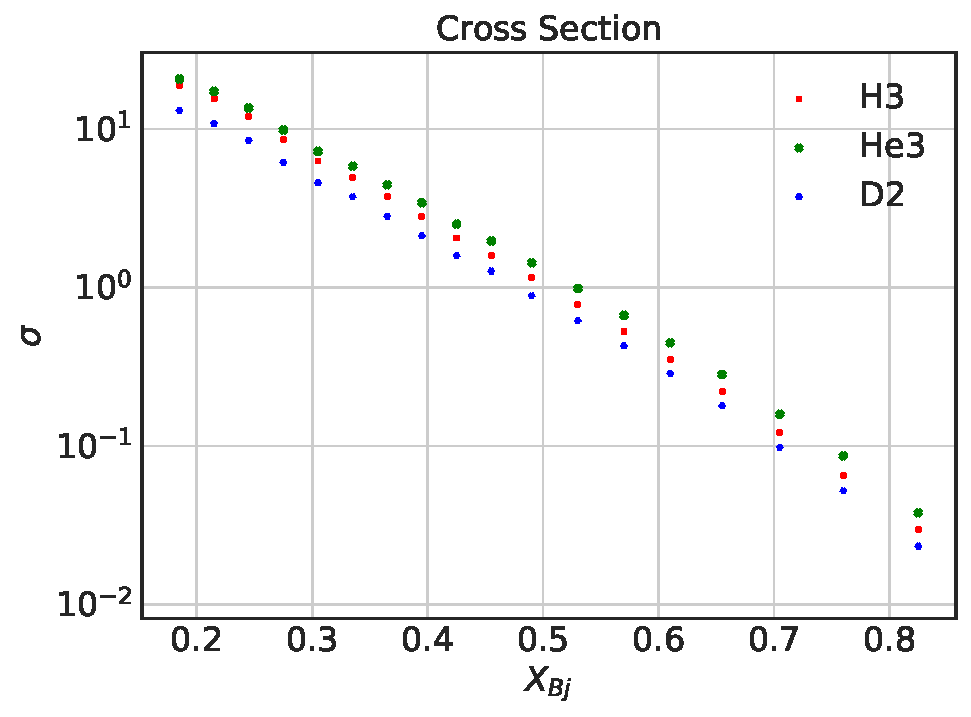
\includegraphics[width=11cm]{../images/Thesis/total_xs.pdf}
\end{figure}

Normalization uncertainty due to target thickness uncertainty\\
$^3$He - 1.12$\%$ $\bullet$ $^3$H - 0.97$\%$ $\bullet$  D - 0.56$\%$
\end{frame}
%----------------------------------------------

\begin{frame}{}

\begin{table}[]
\caption*{Relative uncertatiny contributions for the cross section $^3$H.}
\begin{tabular}{|p{2.2cm}|l|l|l|l|l|l|}
\hline
\multicolumn{1}{|r|}{\textbf{Xbjc}} & \textbf{0.185} & \textbf{0.305} & \textbf{0.49} & \textbf{0.57} & \textbf{0.705} & \textbf{0.825} \\ \hline
\textbf{Yield Error}                & 0.01           & 0.0107         & 0.0149        & 0.0151        & 0.0141         & 0.0163         \\ \hline
Stat Error*                         & 0.0055         & 0.0059         & 0.01          & 0.0111        & 0.0113         & 0.0143         \\ \hline
End Cap*                            & 0.007          & 0.007          & 0.007         & 0.007         & 0.007          & 0.007          \\ \hline
Eff Error*                          & 0.004          & 0.0051         & 0.0083        & 0.0071        & 0.0041         & 0.0032         \\ \hline\hline
\textbf{MC\&Model}                  & 0.016          & 0.014          & 0.013         & 0.016         & 0.03           & 0.037          \\ \hline
Resolution**                        & 0.015          & 0.011          & 0.005         & 0.001         & 0.007          & 0.018          \\ \hline
Model**                             & 0.006          & 0.009          & 0.012         & 0.016         & 0.029          & 0.032          \\ \hline\hline
\textbf{Total Error}                & 0.019          & 0.018          & 0.02          & 0.022         & 0.033          & 0.04           \\ \hline
\end{tabular}

* Largest contributers to the uncertainty in the yield calculation\\
** Largest contributers to the uncertainty in Monte Carlo and Cross section model calculation. 

\end{table}
\end{frame}

\begin{frame}{Cross section model}
\begin{itemize}
	\item Cross section code from Dr. Gaskell

	\item DIS model corrected with an EMC model -Bodek E139
	\begin{itemize}
		\item neutron and proton structure functions from a Hydrogen fit and deuterium fit
		\item proton - 24 parameter fit for background and resonance and 11 parameters OMEGAW fit for F2.
		\item deuterium - 26 parameter fit for background and resonance and 11 parameters OMEGAW fit for F2
	\end{itemize}
	\item EMC - 8th-degree polynomial  with a quadric polynomial in an exponential
	\begin{itemize}
		\item $C = exp( 0.017 + 0.018 \times log(x) + 0.005 \times log(x)^2)$
		\item $\alpha$ is polynomial
		\item EMC correction $= C \times A^{\alpha}$
	\end{itemize}
\end{itemize}
\end{frame}

\begin{frame}{Cross section Models}
\vspace{-1.cm}
\begin{figure}
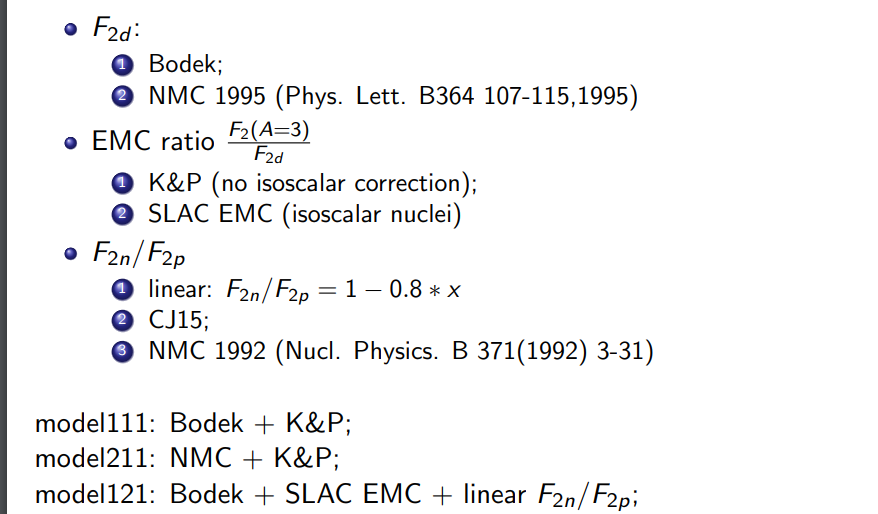
\includegraphics[width=12cm]{../images/models.png}
\end{figure}
\end{frame}

\begin{frame}{Model Cross Section Error}
\vspace{-1.cm}
\begin{figure}
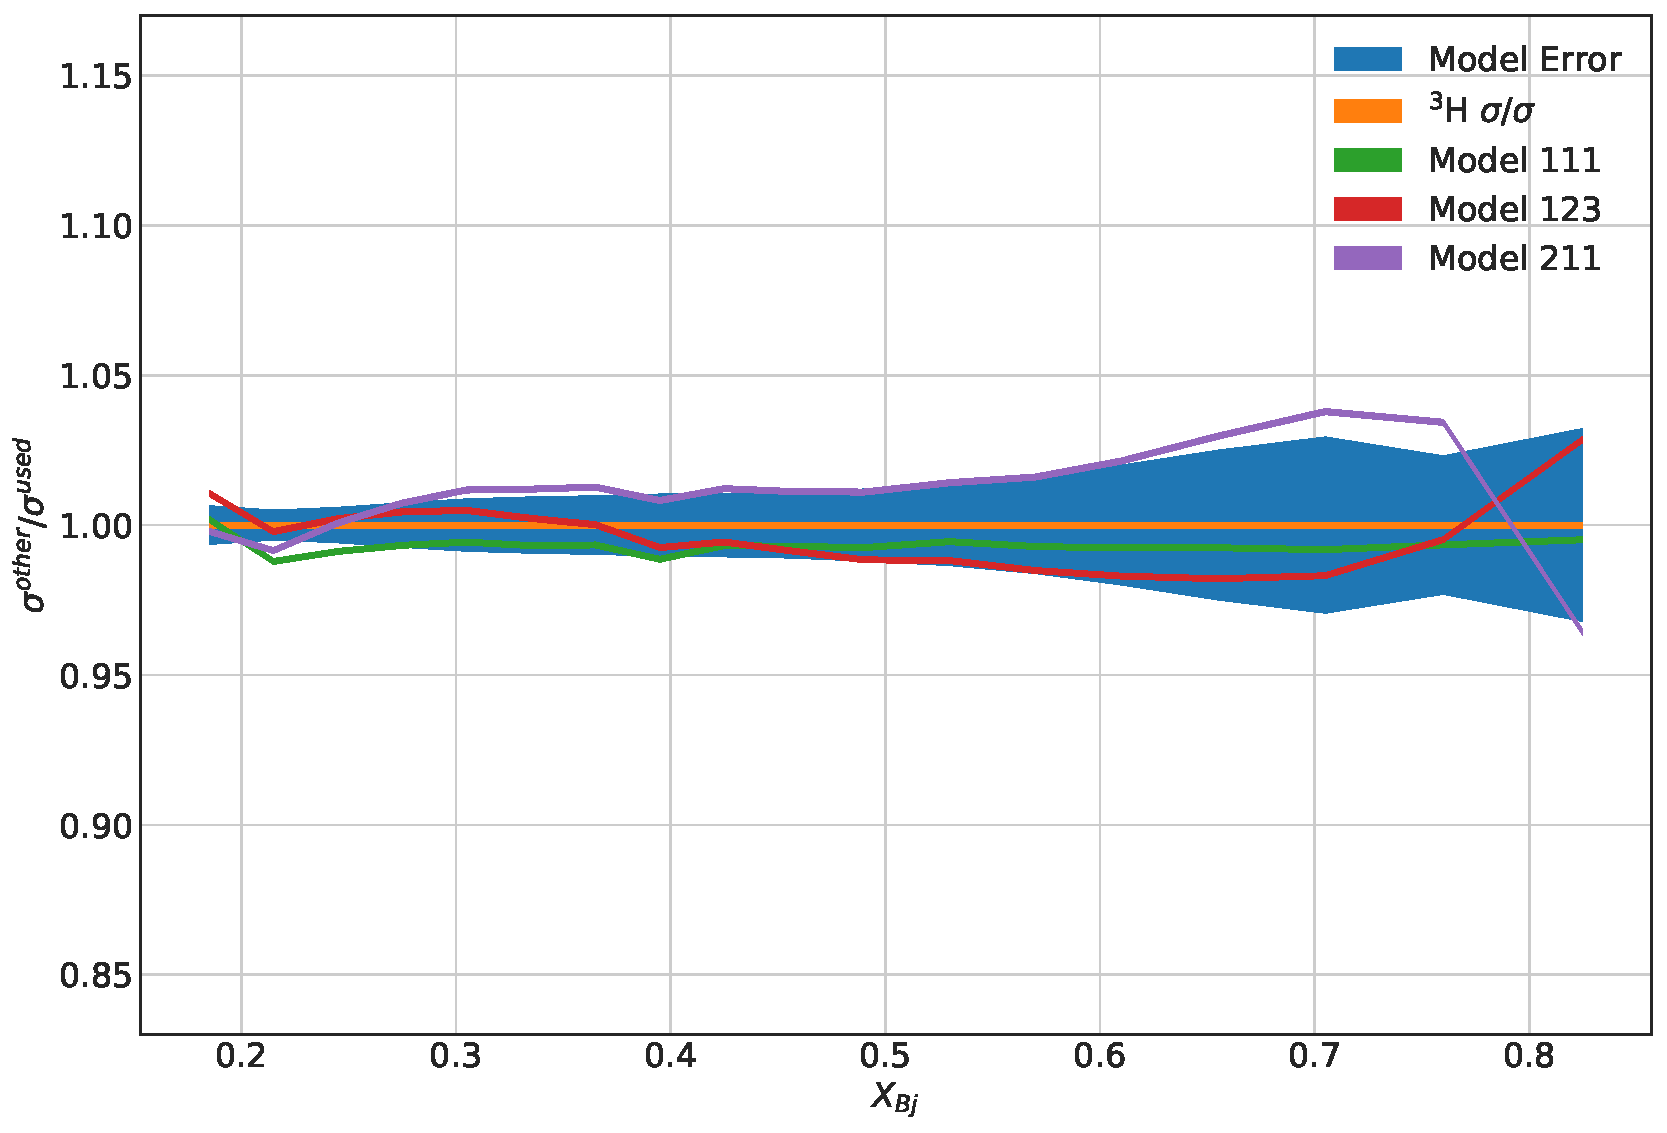
\includegraphics[width=12cm,height=7.5cm]{../images/Mod_err.pdf}
\end{figure}
\end{frame}


\begin{frame}{Model Cross Section Error}
\vspace{-1.cm}
\begin{figure}
\includegraphics[width=12cm,height=7.5cm]{../images/Thesis/cserror.pdf}
\end{figure}
\end{frame}

\begin{frame}{Tacking/Reconstruction Error}
%\vspace{-.5cm}
	$\delta \theta = \pm 0.15\%  \bullet \delta E^{\prime} = \pm 0.025\% \bullet \delta E_{beam} = \pm 0.005\% $\\
	Determine new $Q^2$ and $x_{bj}$ \\
	Calculated new cross sections for extreme situation.
	

	\begin{figure}
		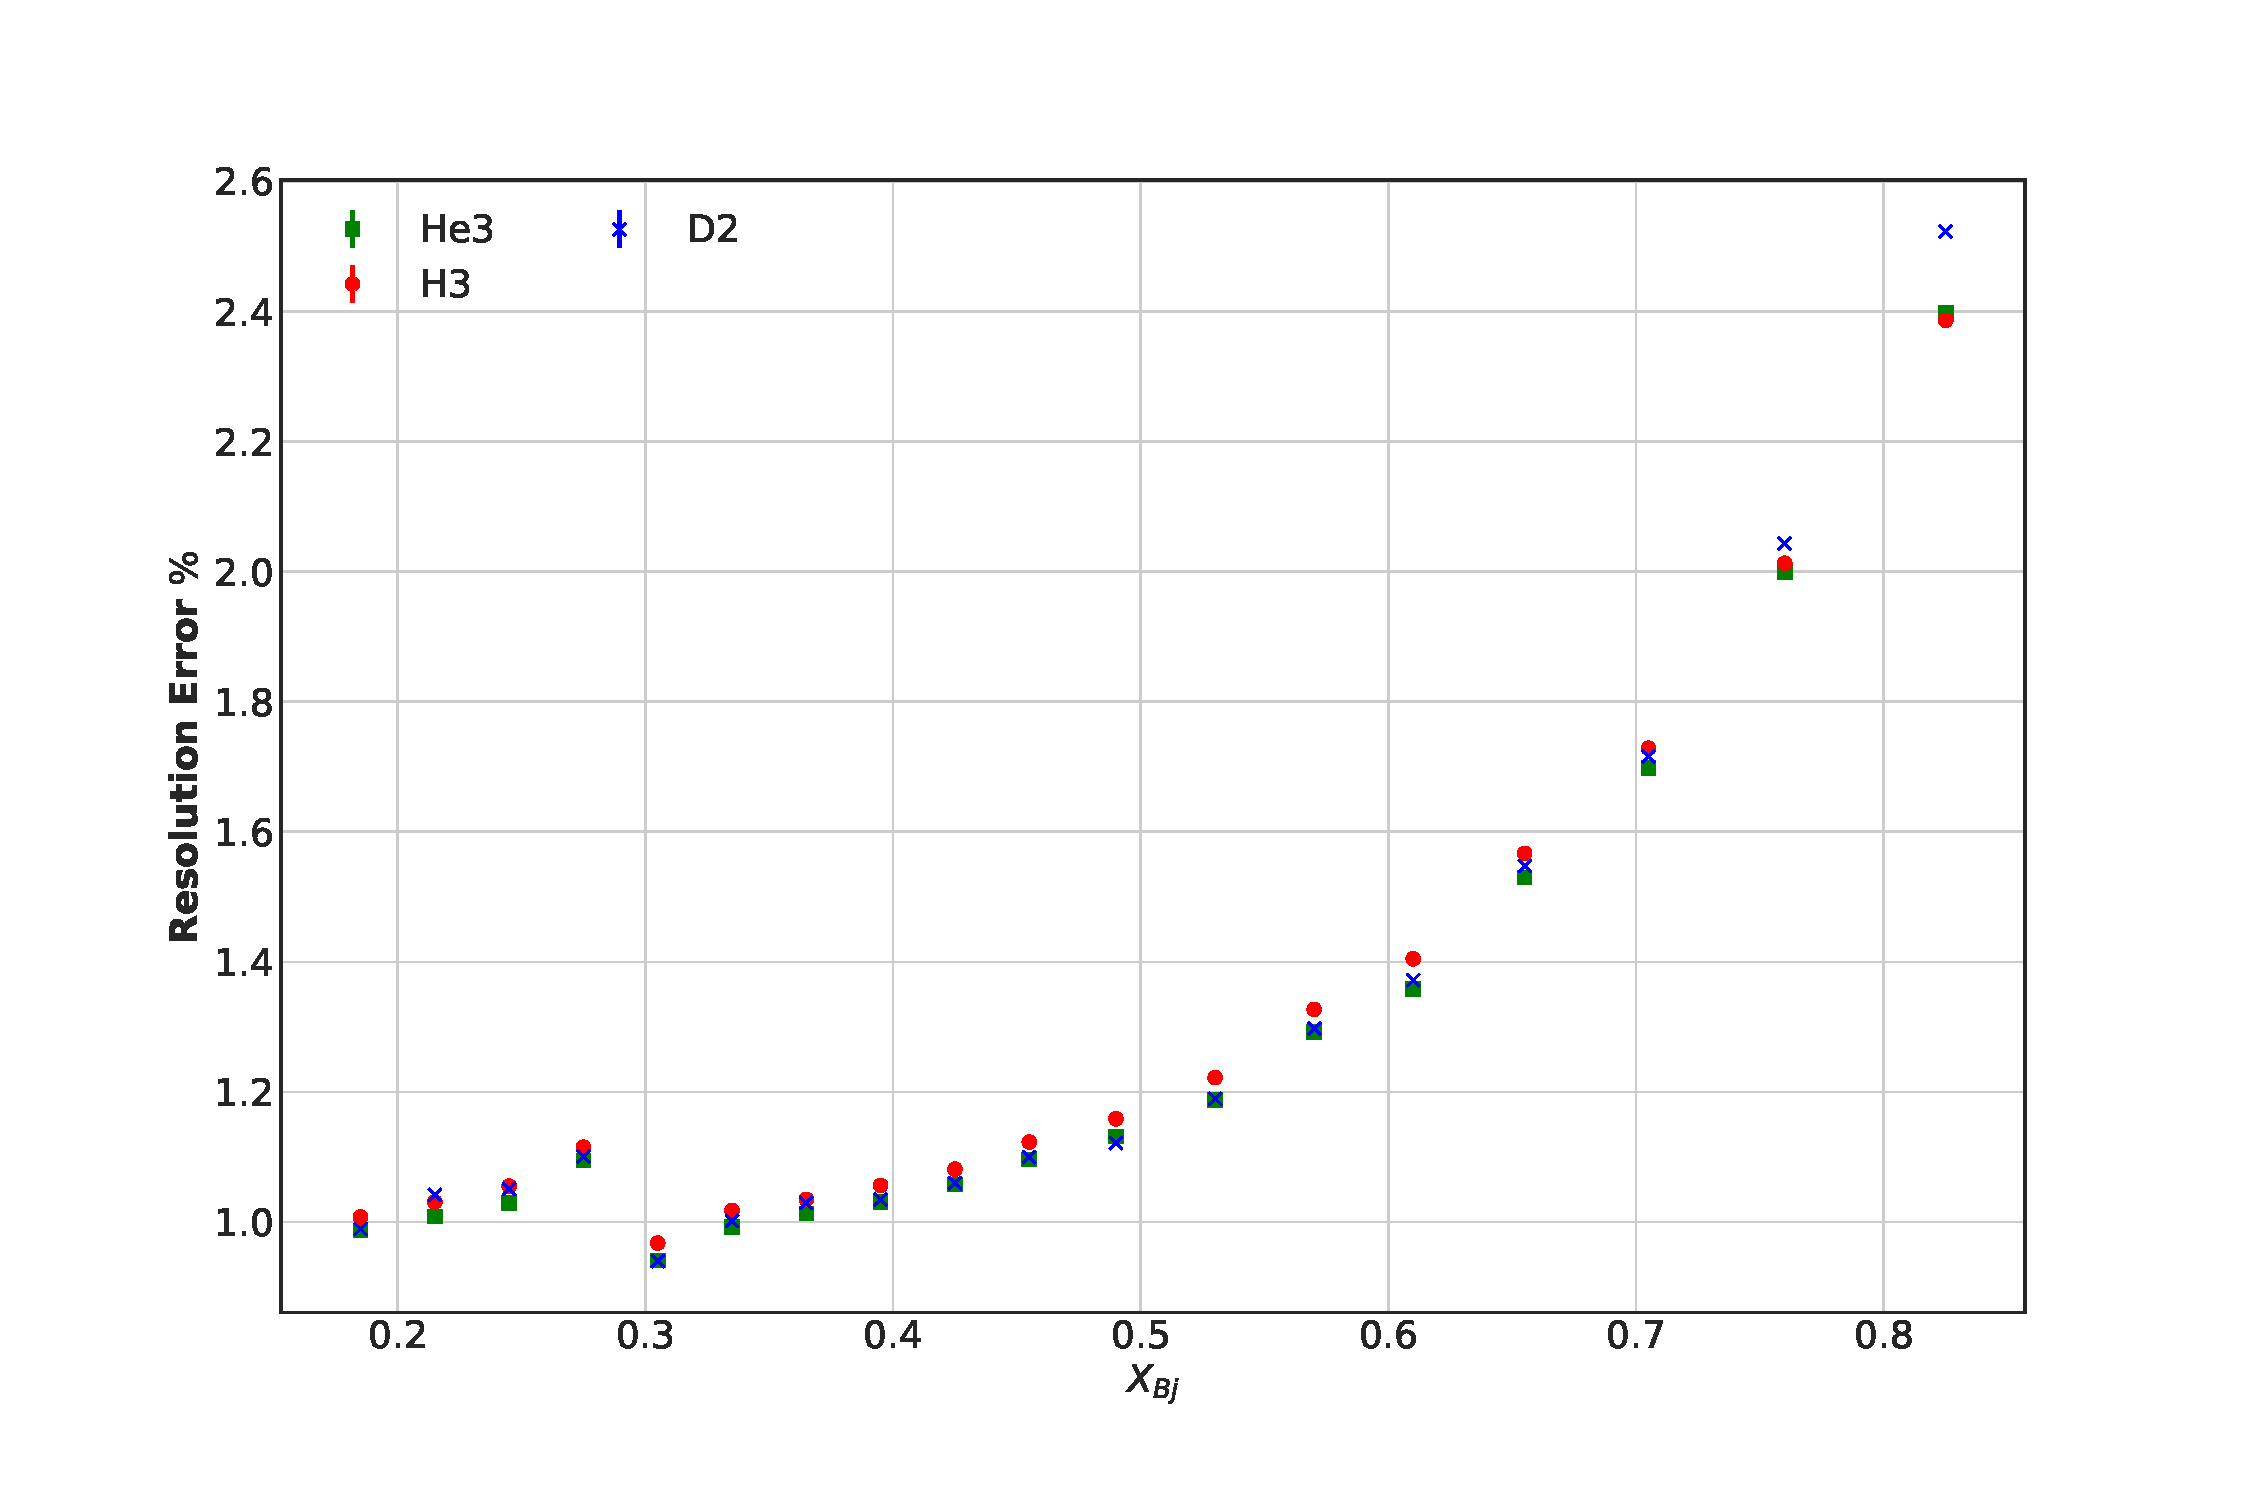
\includegraphics[width=10cm]{../images/Res_err.pdf}
	\end{figure}
\end{frame}



%----------------------------------------------
\begin{frame}{}
\frametitle{Per Nucleon Cross Section Ratio}
\vspace{-8pt}
\begin{figure}
\includegraphics[width=11cm]{../images/Thesis/A_D_ratios.pdf}
\caption*{MARATHON results compared with E03103 \cite{E3103} and the A/D ratios from a DIS scattering model from Arie Bodek model \cite{bodek}.}
\end{figure}

\end{frame}

%----------------------------------------------

\begin{frame}

F$^2$ ratio

\begin{itemize}
\item J.Arrigton.
\begin{itemize}
\item  p=[0.0,0.816,-0.661,0.184,5.509,-0.034,8.714,-0.072,0.450]
\item $(p[1] +  p[2]*epl) + p[3]*np.exp(-p[4]*epl) +  p[5]*np.exp(-p[6]*(1-epl)) + 
p[7]* pow(max(0,epl-p[8]),2)$
\end{itemize}
\item NMC
\begin{itemize}
\item    $AX=0.979-1.692* x+2.797* x^2-4.313* x^3+3.075* x^4$
\item $BX=-0.171* x+0.244* x^2$
\item $F2NP_NMC=AX((Q2/20.0)^{BX})*(1+x^{2}/Q2)$
\end{itemize}
\item K\&P from table
\end{itemize}
\end{frame}



\begin{frame}{Isoscalar Correction Error for $^3$H  }
	\vspace{-.25cm}
	\begin{figure}
		\includegraphics[width=12cm]{../images/Thesis/ISOfacsH3.pdf}
	\end{figure}
\end{frame}

\begin{frame}{Isoscalar Correction Error for $^3$He }
	\vspace{-.25cm}
	\begin{figure}
		\includegraphics[width=12cm]{../images/Thesis/ISOfacsHe3.pdf}
	\end{figure}
\end{frame}

%----------------------------------------------
\begin{frame}{}
$\bullet$ My EMC results for \textcolor{black}{He3 in black} \textcolor{red}{$\bullet$ H3 in red}\\
$\bullet$ \textcolor{ForestGreen}{Previous Jlab He3 in green}
\begin{figure}
\includegraphics[width=10cm]{../images/Thesis/EMC_ratios.pdf}
\caption*{MARATHON results compared with E03103 \cite{E3103} and the EMC ratios from a DIS scattering model from Arie Bodek model \cite{bodek}.}
\end{figure}
\end{frame}

\begin{frame}{EMC results with fits (0.35 - 0.7 in x)}
	\vspace{-20pt}
	\begin{figure}
		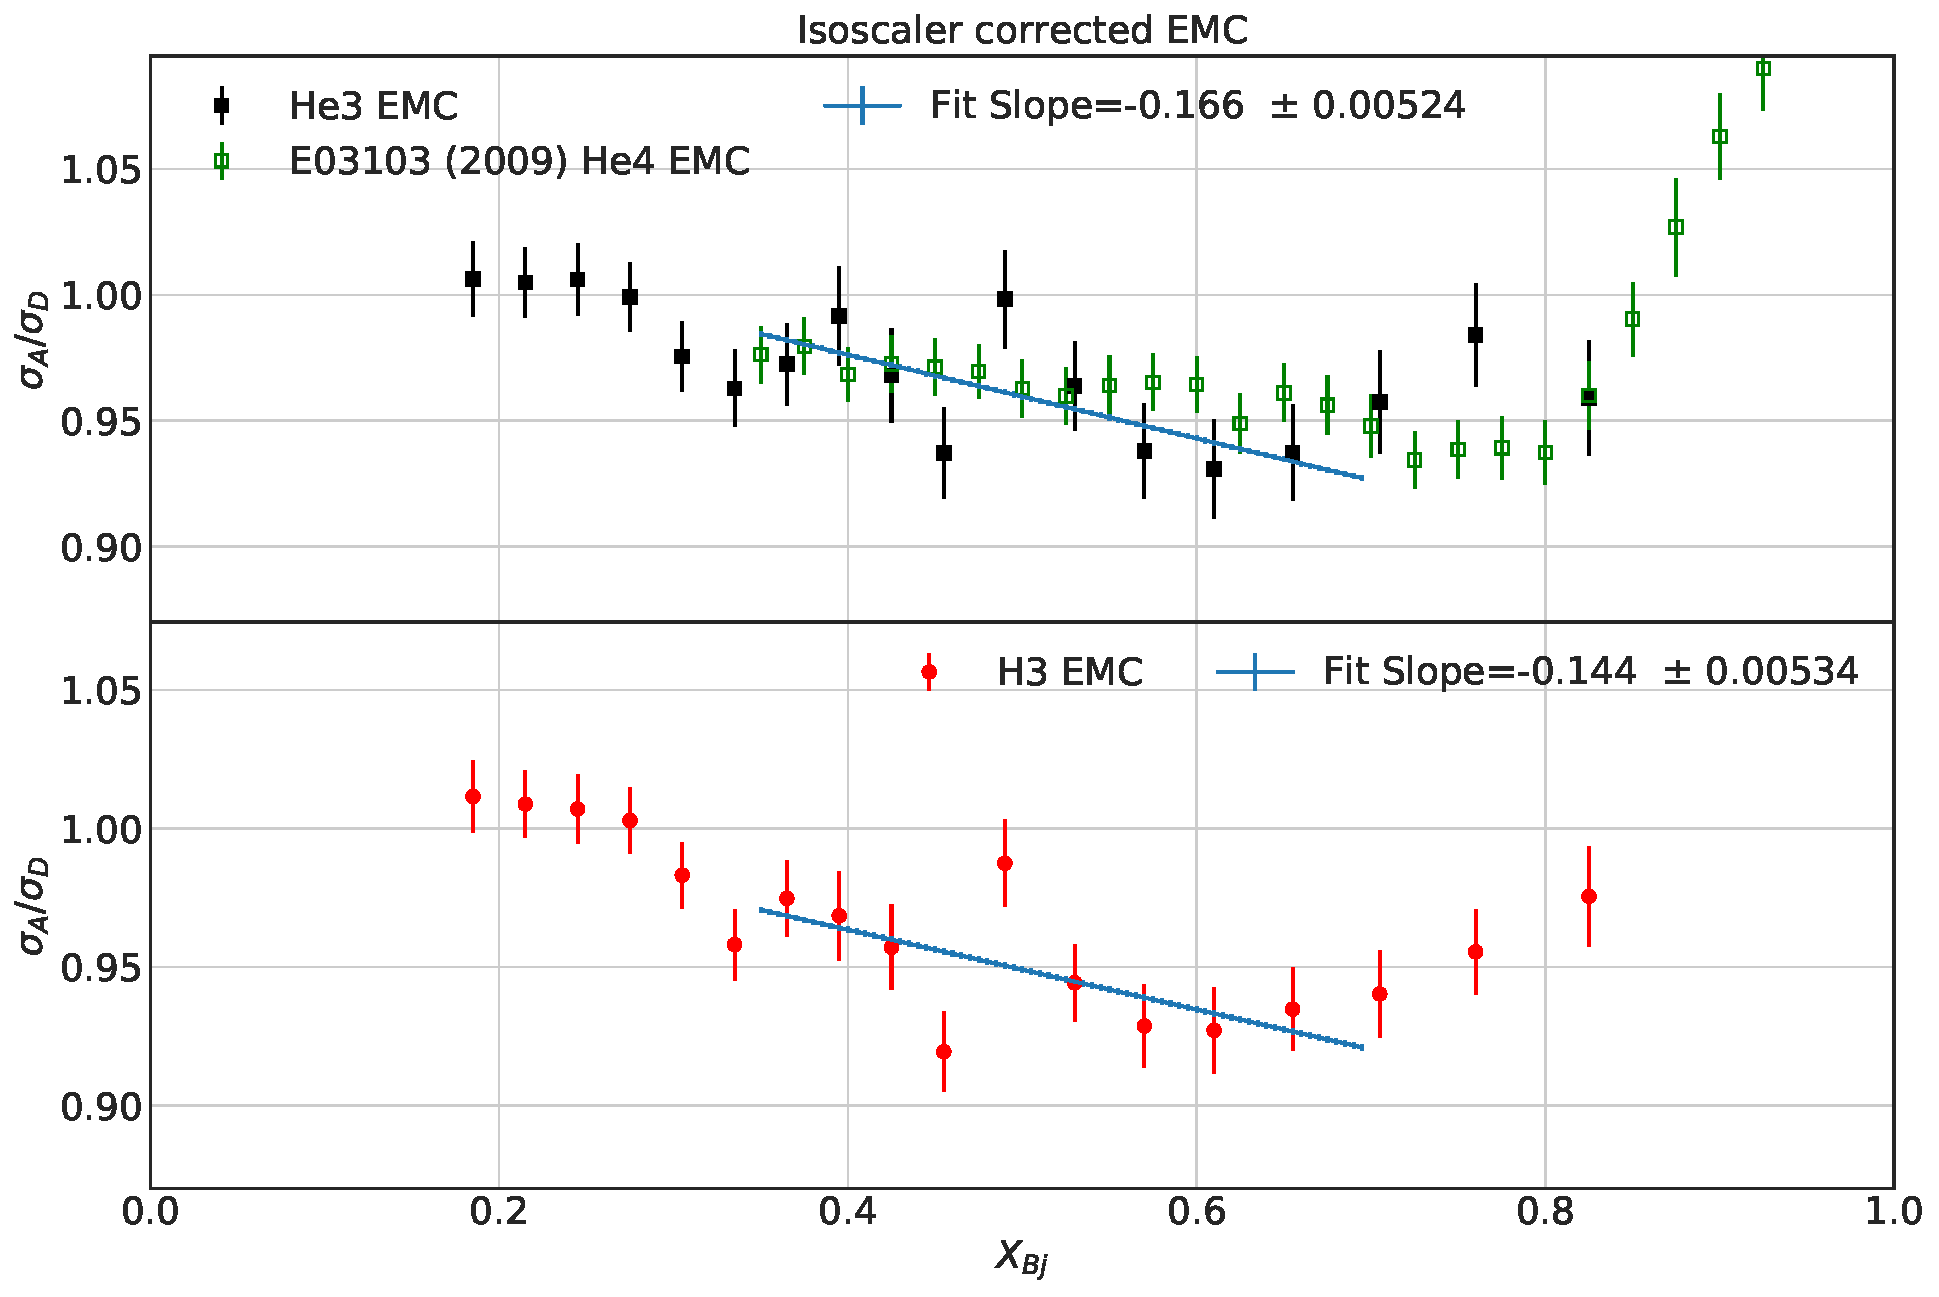
\includegraphics[width=12cm]{../images/EMCfits.pdf}
		\caption*{Ratio of EMC effects.}
	\end{figure}
\end{frame}




\begin{frame}{Ratio of $^3$H/$^3$He EMC effects}
\vspace{-20pt}
\begin{figure}
\includegraphics[width=12cm]{../images/Thesis/A_ratios.pdf}
\caption*{Ratio of EMC effects.}
\end{figure}
\end{frame}







\begin{frame}[allowframebreaks]
\vspace*{-3pt}
\frametitle{References}
\footnotesize{
\begin{thebibliography}{9} % Beamer does not support BibTeX so references must be inserted manually as below
\vspace*{-20pt}
\bibitem[A. Bodek and U.K. Yang, 2002]{bodek} A. Bodek and U.K. Yang
\newblock \emph{Nuclear Physics B, Procc. Suppl. 112 (2002) 70-76 }			
\vspace*{-8pt}				
\bibitem[J.Seely, A. Daniel et al, 2009]{E3103} J. Seely, A. Daniel et al  
\newblock \emph{Phys.\ Rev.\ Lett.\   103, 202301 (2009)}.
\bibitem[J. Arrington, F. Coester, R.J. Holt, T.-S.H. Lee 2008]{JA} J. Arrington, F. Coester, R.J. Holt, T.-S.H. Lee (Argonne, PHY)\newblock Neutron Structure Functions, May 2008, J.Phys. G36 (2009) 025005
DOI: 10.1088/0954-3899/36/2/025005


\end{thebibliography}
}
\end{frame}

\end{document}
